\documentclass{article}

\usepackage{graphicx}
\usepackage{booktabs}
\usepackage{array}
\usepackage{multirow}
\usepackage{siunitx}
\usepackage{pgfplotstable}
\sisetup{
	round-mode= places,
	round-precision= 2,
}

\begin{document}
	\section{Logic Gates}
	Logic gates perform logical operations that take binary input (o's and 1s) and produce a single binary output. They are used in most electronic device including:
	\begin{table}[h!]
		\begin{center}
			\caption{Logic Gates}
			\label{tab:table1}
			\begin{tabular}{|l|c|c|}
				\hline
				Smartphones
				&
				Tablets
				&
				Memory Devices
				\\
				\hline
				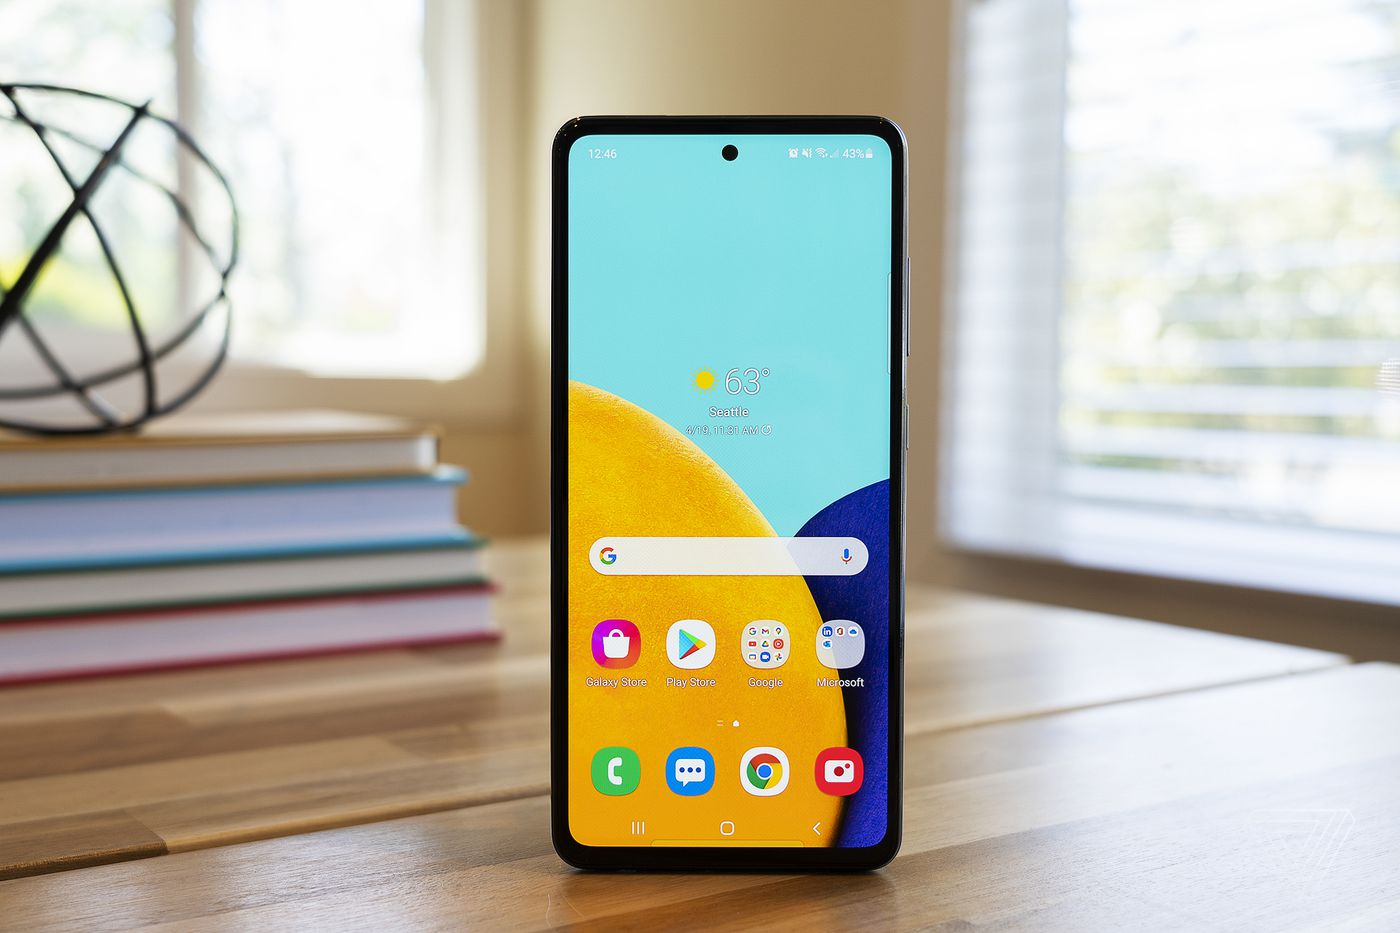
\includegraphics[width=0.2\linewidth]{Picture2}
				&
				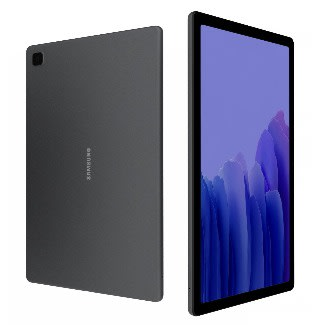
\includegraphics[width=0.25\linewidth]{Picture3}
				&
				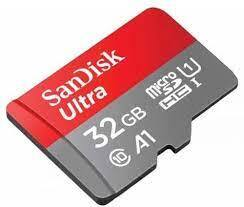
\includegraphics[width=0.2\linewidth]{Picture4}
				\\
				\hline
				\end{tabular}
		\end{center}
		\end{table}
	\newpage
	\section{Github}
	\begin{table}[h!]
		\centering
		\begin{tabular}{| c | m{5cm} | m{5cm} | }
			\hline
			my.github & Advantages & Disadvantages \\ \hline
			\begin{minipage}{.4\textwidth}
				
\includegraphics[width=\linewidth, height=40mm]{Github}
			\end{minipage}
		&
		%\begin{minipage}[t]{5cm}
		\begin{itemize}
			\item Easy to contribute to your source projects
			\item Documentation
			\item showcase your work \ldots
			\item Track changes in your code across versions
			\item Integration options
		\end{itemize}
	%\end{minipage}
	&
	%\begin{minipage}{5cm}
		\begin{itemize}
			\item Continuos integration leads to problems
			\item Not an easy tool for beginners.
			\item Workking with larger files can be tricky
		\end{itemize}
	%\end{minipage}
	\\ \hline
	\end{tabular}
\caption{Github Analysis}\label{tbl:mygithub}
	\end{table}
\newpage
\begin{table}[h!]
	\begin{center}
		\caption{Autogenerated table from .csv file.}
		\label{table1}
		\pgfplotstabletypeset[
		multicolumn names, % allows to have multicolumn names
		col sep=comma, %the separator in our .csv file
		display columns/0/.style={
			column name=$value 1$,
			column type={S},string type},
		display columns/1/.style={
			column name=$Value 2$,
			column type={S},string type},
		every head row/.style={
			before row={\toprule}, % have a rule at top
			after row={
				\si{\ampere} & \si{\volt}\\ % the units separated by &
				\midrule} % rule under units
			},
		every last row/.style={after row=\bottomrule}, % rule at bottom
				]{table.csv} % filename/path to file
	\end{center}
\end{table}
\begin{table}[h!]
	\begin{center}
		\caption{Multirow table}
		\label{tab:table1}
		\begin{tabular}{l|S|r}
			\hline
		\textbf{Value 1} & \textbf{Value 2} & \textbf{Value 3}\\
		$\alpha$ & $\beta$ & $\gamma$ \\
		\hline
		14 & 25.113231 &
		\multirow{2}{*}{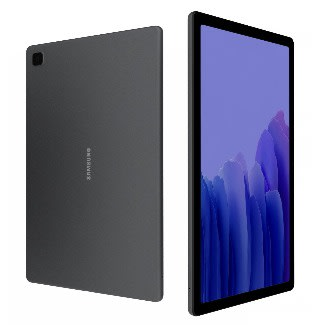
\includegraphics[width=0.07\linewidth]{Picture3}}\\
		25 & 345.113231 & \\
		\hline
		36 & 35.123531 & c \\
		\hline
		\end{tabular}
	\end{center}
\end{table}


\begin{table}[h!]
	\begin{center}
		\caption{Multirow table}
		\label{tab:table1}
		\begin{tabular}{l|S|r}
			\hline 
			\textbf{Value 1} & \textbf{Value 2} & \textbf{Value 3}\\
			$\alpha$ & $\beta$ & $\gamma$ \\
			\hline
			\multicolumn{2}{|c|}{12} & a\\
			\hline\multicolumn{3}{|c|}{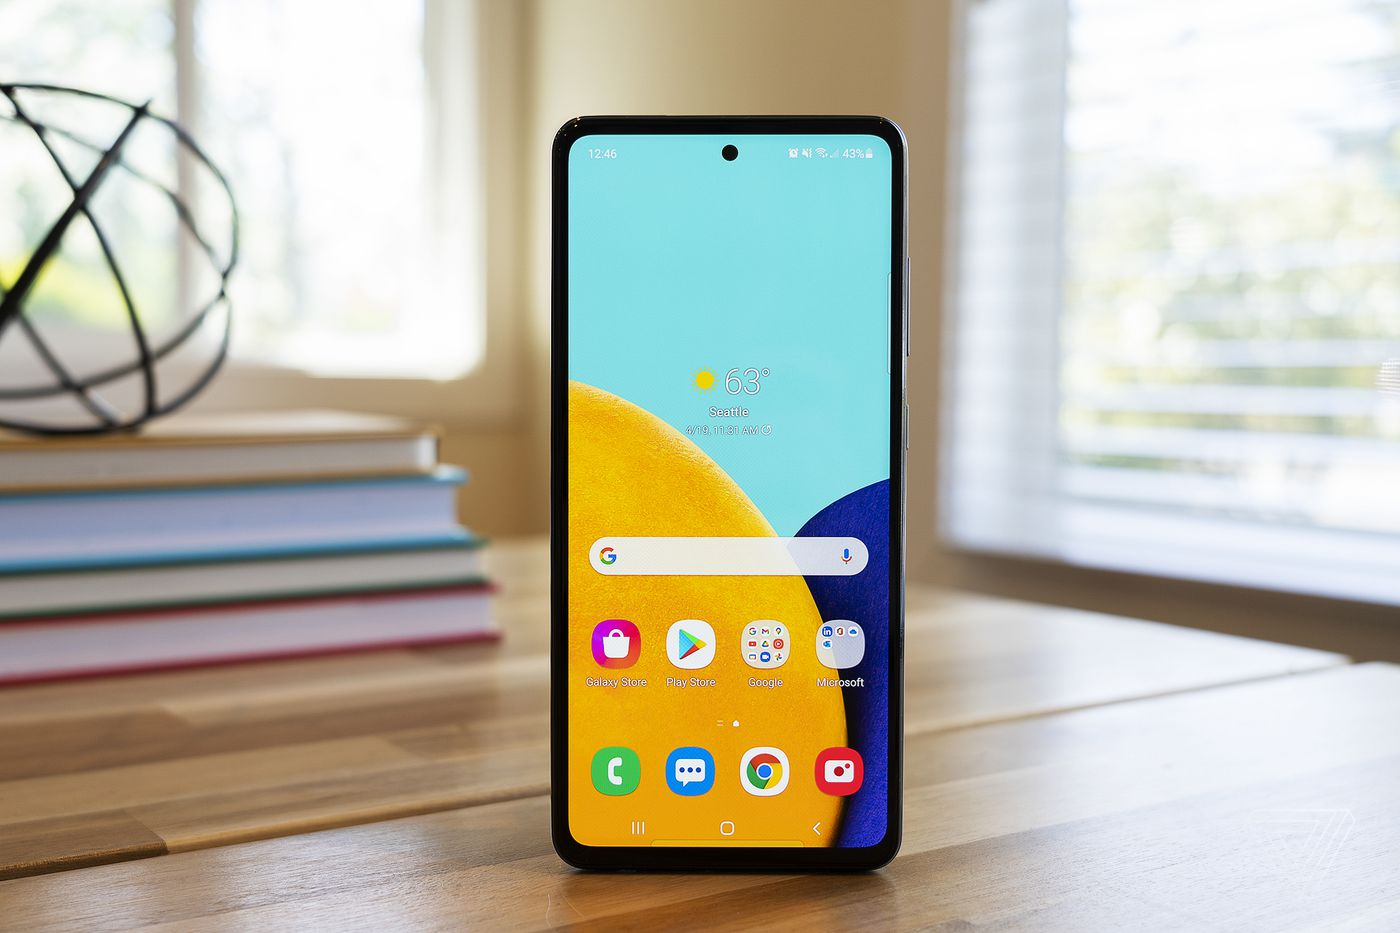
\includegraphics[width=0.15\linewidth]{Picture2}}
			\\
			\hline
			4 & 25.113231 & d\\
			\hline
		\end{tabular}
	\end{center}
\end{table}


\end{document}